\cotefile{29}
\scanpage{115}
phisme évident
\margin{\figure{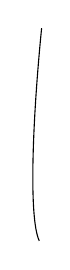
\begin{tikzpicture}\draw (.03,0) .. controls (-.08,-1.1) and (-.14,-2.4) .. (0,-2.7);\end{tikzpicture}}}
\[
\handwritten{\pi}_1^t(U_t)\handwritten{\rightarrow}\handwritten{\pi}_1^t(U)
\]
(un point-base géométrique de $U_t$ étant choisi). Cet homomorphisme est \uline{surjectif}.

Démonstration. Lorsqu'on remplace $L_t$ par $L_{t'}$ générique, alors la conclusion est contenue dans le corollaire 3, en d'autres termes, si $\unsure{\mathbb{U}|\deleted{V}U|\deleted{U}V|\mathbb{V}}$ est un revêtement étale \inserted{connexe} de $U$ \deleted{\unsure{tel que sa,}} (satisfaisant la condition de modération en\unsure{\deleted{g}v|\deleted{v}g}isagée - en fait, ce n'est pas nécessaire, enx vertu de 3 ) alors sa restriction $V_{t'}$ au dessus de $U_{t'}$ est connexe. On veut prouver que sa restriction $V_t$ au dessus de $U_t$ est \inserted{\handwritten{également}} connexe. Or pour un paramètre variable sur \inserted{\handwritten{un voisinage ouvert assez petit $T$ de}} la grassmanienne $\deleted{\unsure{T|G}}$ des $L_{t\handwritten{'}}$\handwritten{,} \deleted{et voisin de $t$, la famill} \inserted{\handwritten{la}} famille des $Y_{t'}$ est un morphisme propre et lisse $Y\handwritten{\rightarrow}T$, et celle des $D_{t'}$ est un sous-schéma fermé \deleted{de} $\handwritten{\Delta}$ de $Y$, qui est la réunion d'un sous-schéma $\handwritten{\Delta}_1$ qui est de codi\unsure{\deleted{emen}mens|\deleted{mens}emen}ion $\handwritten{\geq}2$ sur chaque fibre (et qui ne comp\unsure{\deleted{t}|t}e\inserted{\handwritten{\unsure{m|nt|n}}} pas, à cause du théorème de pureté relative) et d'un diviseur $\handwritten{\Delta_2}$ à croise\unsure{\`{m}|\deleted{à}m|\deleted{m}à|\deleted{è}m|\deleted{m}è}ents normaux relatifs. Le revêtement donné $V$ de $U$ définit un revêtement \deleted{$\unsure{V|U}$ de $Y$} $V'$ de $U'=Y-\handwritten{\Delta}$, et il\deleted{f} faut montrer que la restriction de celui-ci à la fibre géométrique de $t$ est connexe, sachant qu'il en est ainsi de sa restriction à la fibre géométrique en $t'$, la générisation maximale de $t$. Or par la pureté, on sait que $V'$ se prolonge en un revêtement étale $V''$ de $U''=Y-\handwritten{\Delta_2}$, et par hypothèse ce dernier est modérément ramifié sur les fibres, relativement au diviseur $\handwritten{\Delta_2}$. La conclusion est alors une conséquence du théorème \deleted{\unsure{connu}} de spécialisation pour le groupe fondamental modéré, qui figure(ra) dans SGA 1 XIII (exposé de Mme Raynaud).

\uline{Remarque}7.Avec les notations de SGA 7 XVII\deleted{,}I\handwritten{,} 6 s'applique pour tout pinceau de Lefschetz $D$ pour fournir la surjectivité de\deleted{s quotients par}
% archive sheet number: 114
